
%% bare_conf.tex
%% V1.4b
%% 2015/08/26
%% by Michael Shell
%% See:
%% http://www.michaelshell.org/
%% for current contact information.
%%
%% This is a skeleton file demonstrating the use of IEEEtran.cls
%% (requires IEEEtran.cls version 1.8b or later) with an IEEE
%% conference paper.
%%
%% Support sites:
%% http://www.michaelshell.org/tex/ieeetran/
%% http://www.ctan.org/pkg/ieeetran
%% and
%% http://www.ieee.org/

%%*************************************************************************
%% Legal Notice:
%% This code is offered as-is without any warranty either expressed or
%% implied; without even the implied warranty of MERCHANTABILITY or
%% FITNESS FOR A PARTICULAR PURPOSE! 
%% User assumes all risk.
%% In no event shall the IEEE or any contributor to this code be liable for
%% any damages or losses, including, but not limited to, incidental,
%% consequential, or any other damages, resulting from the use or misuse
%% of any information contained here.
%%
%% All comments are the opinions of their respective authors and are not
%% necessarily endorsed by the IEEE.
%%
%% This work is distributed under the LaTeX Project Public License (LPPL)
%% ( http://www.latex-project.org/ ) version 1.3, and may be freely used,
%% distributed and modified. A copy of the LPPL, version 1.3, is included
%% in the base LaTeX documentation of all distributions of LaTeX released
%% 2003/12/01 or later.
%% Retain all contribution notices and credits.
%% ** Modified files should be clearly indicated as such, including  **
%% ** renaming them and changing author support contact information. **
%%*************************************************************************


% *** Authors should verify (and, if needed, correct) their LaTeX system  ***
% *** with the testflow diagnostic prior to trusting their LaTeX platform ***
% *** with production work. The IEEE's font choices and paper sizes can   ***
% *** trigger bugs that do not appear when using other class files.       ***                          ***
% The testflow support page is at:
% http://www.michaelshell.org/tex/testflow/



\documentclass[conference]{IEEEtran}
% Some Computer Society conferences also require the compsoc mode option,
% but others use the standard conference format.
%
% If IEEEtran.cls has not been installed into the LaTeX system files,
% manually specify the path to it like:
%\documentclass[conference]{../sty/IEEEtran}





% Some very useful LaTeX packages include:
% (uncomment the ones you want to load)


% *** MISC UTILITY PACKAGES ***
%
%\usepackage{ifpdf}
% Heiko Oberdiek's ifpdf.sty is very useful if you need conditional
% compilation based on whether the output is pdf or dvi.
% usage:
% \ifpdf
%   % pdf code
% \else
%   % dvi code
% \fi
% The latest version of ifpdf.sty can be obtained from:
% http://www.ctan.org/pkg/ifpdf
% Also, note that IEEEtran.cls V1.7 and later provides a builtin
% \ifCLASSINFOpdf conditional that works the same way.
% When switching from latex to pdflatex and vice-versa, the compiler may
% have to be run twice to clear warning/error messages.






% *** CITATION PACKAGES ***
%
%\usepackage{cite}
% cite.sty was written by Donald Arseneau
% V1.6 and later of IEEEtran pre-defines the format of the cite.sty package
% \cite{} output to follow that of the IEEE. Loading the cite package will
% result in citation numbers being automatically sorted and properly
% "compressed/ranged". e.g., [1], [9], [2], [7], [5], [6] without using
% cite.sty will become [1], [2], [5]--[7], [9] using cite.sty. cite.sty's
% \cite will automatically add leading space, if needed. Use cite.sty's
% noadjust option (cite.sty V3.8 and later) if you want to turn this off
% such as if a citation ever needs to be enclosed in parenthesis.
% cite.sty is already installed on most LaTeX systems. Be sure and use
% version 5.0 (2009-03-20) and later if using hyperref.sty.
% The latest version can be obtained at:
% http://www.ctan.org/pkg/cite
% The documentation is contained in the cite.sty file itself.






% *** GRAPHICS RELATED PACKAGES ***
%
\ifCLASSINFOpdf
  % \usepackage[pdftex]{graphicx}
  % declare the path(s) where your graphic files are
  % \graphicspath{{../pdf/}{../jpeg/}}
  % and their extensions so you won't have to specify these with
  % every instance of \includegraphics
  % \DeclareGraphicsExtensions{.pdf,.jpeg,.png}
\else
  % or other class option (dvipsone, dvipdf, if not using dvips). graphicx
  % will default to the driver specified in the system graphics.cfg if no
  % driver is specified.
  % \usepackage[dvips]{graphicx}
  % declare the path(s) where your graphic files are
  % \graphicspath{{../eps/}}
  % and their extensions so you won't have to specify these with
  % every instance of \includegraphics
  % \DeclareGraphicsExtensions{.eps}
\fi
% graphicx was written by David Carlisle and Sebastian Rahtz. It is
% required if you want graphics, photos, etc. graphicx.sty is already
% installed on most LaTeX systems. The latest version and documentation
% can be obtained at: 
% http://www.ctan.org/pkg/graphicx
% Another good source of documentation is "Using Imported Graphics in
% LaTeX2e" by Keith Reckdahl which can be found at:
% http://www.ctan.org/pkg/epslatex
%
% latex, and pdflatex in dvi mode, support graphics in encapsulated
% postscript (.eps) format. pdflatex in pdf mode supports graphics
% in .pdf, .jpeg, .png and .mps (metapost) formats. Users should ensure
% that all non-photo figures use a vector format (.eps, .pdf, .mps) and
% not a bitmapped formats (.jpeg, .png). The IEEE frowns on bitmapped formats
% which can result in "jaggedy"/blurry rendering of lines and letters as
% well as large increases in file sizes.
%
% You can find documentation about the pdfTeX application at:
% http://www.tug.org/applications/pdftex





% *** MATH PACKAGES ***
%
%\usepackage{amsmath}
% A popular package from the American Mathematical Society that provides
% many useful and powerful commands for dealing with mathematics.
%
% Note that the amsmath package sets \interdisplaylinepenalty to 10000
% thus preventing page breaks from occurring within multiline equations. Use:
%\interdisplaylinepenalty=2500
% after loading amsmath to restore such page breaks as IEEEtran.cls normally
% does. amsmath.sty is already installed on most LaTeX systems. The latest
% version and documentation can be obtained at:
% http://www.ctan.org/pkg/amsmath





% *** SPECIALIZED LIST PACKAGES ***
%
%\usepackage{algorithmic}
% algorithmic.sty was written by Peter Williams and Rogerio Brito.
% This package provides an algorithmic environment fo describing algorithms.
% You can use the algorithmic environment in-text or within a figure
% environment to provide for a floating algorithm. Do NOT use the algorithm
% floating environment provided by algorithm.sty (by the same authors) or
% algorithm2e.sty (by Christophe Fiorio) as the IEEE does not use dedicated
% algorithm float types and packages that provide these will not provide
% correct IEEE style captions. The latest version and documentation of
% algorithmic.sty can be obtained at:
% http://www.ctan.org/pkg/algorithms
% Also of interest may be the (relatively newer and more customizable)
% algorithmicx.sty package by Szasz Janos:
% http://www.ctan.org/pkg/algorithmicx




% *** ALIGNMENT PACKAGES ***
%
%\usepackage{array}
% Frank Mittelbach's and David Carlisle's array.sty patches and improves
% the standard LaTeX2e array and tabular environments to provide better
% appearance and additional user controls. As the default LaTeX2e table
% generation code is lacking to the point of almost being broken with
% respect to the quality of the end results, all users are strongly
% advised to use an enhanced (at the very least that provided by array.sty)
% set of table tools. array.sty is already installed on most systems. The
% latest version and documentation can be obtained at:
% http://www.ctan.org/pkg/array


% IEEEtran contains the IEEEeqnarray family of commands that can be used to
% generate multiline equations as well as matrices, tables, etc., of high
% quality.




% *** SUBFIGURE PACKAGES ***
%\ifCLASSOPTIONcompsoc
%  \usepackage[caption=false,font=normalsize,labelfont=sf,textfont=sf]{subfig}
%\else
%  \usepackage[caption=false,font=footnotesize]{subfig}
%\fi
% subfig.sty, written by Steven Douglas Cochran, is the modern replacement
% for subfigure.sty, the latter of which is no longer maintained and is
% incompatible with some LaTeX packages including fixltx2e. However,
% subfig.sty requires and automatically loads Axel Sommerfeldt's caption.sty
% which will override IEEEtran.cls' handling of captions and this will result
% in non-IEEE style figure/table captions. To prevent this problem, be sure
% and invoke subfig.sty's "caption=false" package option (available since
% subfig.sty version 1.3, 2005/06/28) as this is will preserve IEEEtran.cls
% handling of captions.
% Note that the Computer Society format requires a larger sans serif font
% than the serif footnote size font used in traditional IEEE formatting
% and thus the need to invoke different subfig.sty package options depending
% on whether compsoc mode has been enabled.
%
% The latest version and documentation of subfig.sty can be obtained at:
% http://www.ctan.org/pkg/subfig




% *** FLOAT PACKAGES ***
%
%\usepackage{fixltx2e}
% fixltx2e, the successor to the earlier fix2col.sty, was written by
% Frank Mittelbach and David Carlisle. This package corrects a few problems
% in the LaTeX2e kernel, the most notable of which is that in current
% LaTeX2e releases, the ordering of single and double column floats is not
% guaranteed to be preserved. Thus, an unpatched LaTeX2e can allow a
% single column figure to be placed prior to an earlier double column
% figure.
% Be aware that LaTeX2e kernels dated 2015 and later have fixltx2e.sty's
% corrections already built into the system in which case a warning will
% be issued if an attempt is made to load fixltx2e.sty as it is no longer
% needed.
% The latest version and documentation can be found at:
% http://www.ctan.org/pkg/fixltx2e


%\usepackage{stfloats}
% stfloats.sty was written by Sigitas Tolusis. This package gives LaTeX2e
% the ability to do double column floats at the bottom of the page as well
% as the top. (e.g., "\begin{figure*}[!b]" is not normally possible in
% LaTeX2e). It also provides a command:
%\fnbelowfloat
% to enable the placement of footnotes below bottom floats (the standard
% LaTeX2e kernel puts them above bottom floats). This is an invasive package
% which rewrites many portions of the LaTeX2e float routines. It may not work
% with other packages that modify the LaTeX2e float routines. The latest
% version and documentation can be obtained at:
% http://www.ctan.org/pkg/stfloats
% Do not use the stfloats baselinefloat ability as the IEEE does not allow
% \baselineskip to stretch. Authors submitting work to the IEEE should note
% that the IEEE rarely uses double column equations and that authors should try
% to avoid such use. Do not be tempted to use the cuted.sty or midfloat.sty
% packages (also by Sigitas Tolusis) as the IEEE does not format its papers in
% such ways.
% Do not attempt to use stfloats with fixltx2e as they are incompatible.
% Instead, use Morten Hogholm'a dblfloatfix which combines the features
% of both fixltx2e and stfloats:
%
% \usepackage{dblfloatfix}
% The latest version can be found at:
% http://www.ctan.org/pkg/dblfloatfix




% *** PDF, URL AND HYPERLINK PACKAGES ***
%
%\usepackage{url}
% url.sty was written by Donald Arseneau. It provides better support for
% handling and breaking URLs. url.sty is already installed on most LaTeX
% systems. The latest version and documentation can be obtained at:
% http://www.ctan.org/pkg/url
% Basically, \url{my_url_here}.




% *** Do not adjust lengths that control margins, column widths, etc. ***
% *** Do not use packages that alter fonts (such as pslatex).         ***
% There should be no need to do such things with IEEEtran.cls V1.6 and later.
% (Unless specifically asked to do so by the journal or conference you plan
% to submit to, of course. )
\usepackage{graphicx}
\usepackage{natbib} 

% correct bad hyphenation here
\hyphenation{op-tical net-works semi-conduc-tor}


\usepackage{amsmath}
\begin{document}

%
% paper title
% Titles are generally capitalized except for words such as a, an, and, as,
% at, but, by, for, in, nor, of, on, or, the, to and up, which are usually
% not capitalized unless they are the first or last word of the title.
% Linebreaks \\ can be used within to get better formatting as desired.
% Do not put math or special symbols in the title.

\title{Tone Biased MMR Text Summarization}
 

% author names and affiliations
% use a multiple column layout for up to three different
% affiliations

\author{\IEEEauthorblockN{Mayank Chaudhari}
\IEEEauthorblockA{ Department of CS \& IS \\
BITS Pilani- K.K.Birla Goa Campus}\\

\IEEEauthorblockN{Aakash Nelson Mattukoyya}
\IEEEauthorblockA{ Department of CS \& IS \\
BITS Pilani- K.K.Birla Goa Campus}\\

}


% conference papers do not typically use \thanks and this command
% is locked out in conference mode. If really needed, such as for
% the acknowledgment of grants, issue a \IEEEoverridecommandlockouts
% after \documentclass

% for over three affiliations, or if they all won't fit within the width
% of the page, use this alternative format:
% 
%\author{\IEEEauthorblockN{Michael Shell\IEEEauthorrefmark{1},
%Homer Simpson\IEEEauthorrefmark{2},
%James Kirk\IEEEauthorrefmark{3}, 
%Montgomery Scott\IEEEauthorrefmark{3} and
%Eldon Tyrell\IEEEauthorrefmark{4}}
%\IEEEauthorblockA{\IEEEauthorrefmark{1}School of Electrical and Computer Engineering\\
%Georgia Institute of Technology,
%Atlanta, Georgia 30332--0250\\ Email: see http://www.michaelshell.org/contact.html}
%\IEEEauthorblockA{\IEEEauthorrefmark{2}Twentieth Century Fox, Springfield, USA\\
%Email: homer@thesimpsons.com}
%\IEEEauthorblockA{\IEEEauthorrefmark{3}Starfleet Academy, San Francisco, California 96678-2391\\
%Telephone: (800) 555--1212, Fax: (888) 555--1212}
%\IEEEauthorblockA{\IEEEauthorrefmark{4}Tyrell Inc., 123 Replicant Street, Los Angeles, California 90210--4321}}




% use for special paper notices
%\IEEEspecialpapernotice{(Invited Paper)}




% make the title area
\maketitle

% As a general rule, do not put math, special symbols or citations
% in the abstract
\begin{abstract}
Text summarization is an interesting area for researchers to develop new techniques to provide human like summaries for vast amounts of information. Summarization techniques tend to focus on providing accurate representation of content; and often the tone of the content is ignored. Tone of the content sets a baseline for how a reader perceives the content. As such being able to generate summary with tone that is appropriate for the reader is important.\\
 In our project work we implement Maximal Marginal Relevance [MMR] based multi-document text summarization and propose a naïve model to change tone of the summarization by setting a bias to specific set of words and restricting other words in the summarization output. This bias towards a specified set of words produces a summary whose tone is same as tone of specified words. \\\\
\textit{Keywords: }text summarization; maximal marginal relevance; tone bias

\end{abstract}

% no keywords




% For peer review papers, you can put extra information on the cover
% page as needed:
% \ifCLASSOPTIONpeerreview
% \begin{center} \bfseries EDICS Category: 3-BBND \end{center}
% \fi
%
% For peerreview papers, this IEEEtran command inserts a page break and
% creates the second title. It will be ignored for other modes.
\IEEEpeerreviewmaketitle



\section{Introduction}
% no \IEEEPARstart
With vast amounts of information being generated every day, automated text summarization is used to represent such vast information in compact form. There are many techniques that have been developed over recent times to improve the accuracy of summary and provide summaries that are ‘human like’. Various features of sentences are used to rank the sentences which should be included in the summary. The top ranked sentences are refined and reordered to form a coherent summary. Feature based ranking means that we try improving the query relevance of the sentences selected for summarization but this in turn might increase redundancy in summary as many query relevant sentences may have similar content. In our project work we implemented Maximal Marginal Relevance [MMR] based text multi-document summarization which along with sentence ranking considers the novelty of the sentence there by reducing the redundancy in final summarization.
\par
Current summarization techniques try make sure that all information in content is accurately represented in the summary. Such summarization gives us accurate representation of data, however, the summarization isn’t ‘human like’.  Daily life human summaries usually tend to be customized for reader by using bias in the tone of summarization. We propose a naïve model for biasing the tone of summary by using a set of words which have defined polarity tag to decide whether to include or discard the sentence in the summary.
\par
The rest of the report is organized as follows –  Section II gives an overview of current work done in the proposed area. Section III discusses our approach and implementation of MMR multi-document text summarization and Naïve tone biasing. Section IV briefly discusses the applications of tone biasing. Section V we discuss the results and observations obtained by implementing our approach. Section VI describes future scope of our work and conclusions.




% You must have at least 2 lines in the paragraph with the drop letter
% (should never be an issue)

% An example of a floating figure using the graphicx package.
% Note that \label must occur AFTER (or within) \caption.
% For figures, \caption should occur after the \includegraphics.
% Note that IEEEtran v1.7 and later has special internal code that
% is designed to preserve the operation of \label within \caption
% even when the captionsoff option is in effect. However, because
% of issues like this, it may be the safest practice to put all your
% \label just after \caption rather than within \caption{}.
%
% Reminder: the "draftcls" or "draftclsnofoot", not "draft", class
% option should be used if it is desired that the figures are to be
% displayed while in draft mode.
%
%\begin{figure}[!t]
%\centering
%\includegraphics[width=2.5in]{myfigure}
% where an .eps filename suffix will be assumed under latex, 
% and a .pdf suffix will be assumed for pdflatex; or what has been declared
% via \DeclareGraphicsExtensions.
%\caption{Simulation results for the network.}
%\label{fig_sim}
%\end{figure}

% Note that the IEEE typically puts floats only at the top, even when this
% results in a large percentage of a column being occupied by floats.


% An example of a double column floating figure using two subfigures.
% (The subfig.sty package must be loaded for this to work.)
% The subfigure \label commands are set within each subfloat command,
% and the \label for the overall figure must come after \caption.
% \hfil is used as a separator to get equal spacing.
% Watch out that the combined width of all the subfigures on a 
% line do not exceed the text width or a line break will occur.
%
%\begin{figure*}[!t]
%\centering
%\subfloat[Case I]{\includegraphics[width=2.5in]{box}%
%\label{fig_first_case}}
%\hfil
%\subfloat[Case II]{\includegraphics[width=2.5in]{box}%
%\label{fig_second_case}}
%\caption{Simulation results for the network.}
%\label{fig_sim}
%\end{figure*}
%
% Note that often IEEE papers with subfigures do not employ subfigure
% captions (using the optional argument to \subfloat[]), but instead will
% reference/describe all of them (a), (b), etc., within the main caption.
% Be aware that for subfig.sty to generate the (a), (b), etc., subfigure
% labels, the optional argument to \subfloat must be present. If a
% subcaption is not desired, just leave its contents blank,
% e.g., \subfloat[].


% An example of a floating table. Note that, for IEEE style tables, the
% \caption command should come BEFORE the table and, given that table
% captions serve much like titles, are usually capitalized except for words
% such as a, an, and, as, at, but, by, for, in, nor, of, on, or, the, to
% and up, which are usually not capitalized unless they are the first or
% last word of the caption. Table text will default to \footnotesize as
% the IEEE normally uses this smaller font for tables.
% The \label must come after \caption as always.
%
%\begin{table}[!t]
%% increase table row spacing, adjust to taste
%\renewcommand{\arraystretch}{1.3}
% if using array.sty, it might be a good idea to tweak the value of
% \extrarowheight as needed to properly center the text within the cells
%\caption{An Example of a Table}
%\label{table_example}
%\centering
%% Some packages, such as MDW tools, offer better commands for making tables
%% than the plain LaTeX2e tabular which is used here.
%\begin{tabular}{|c||c|}
%\hline
%One & Two\\
%\hline
%Three & Four\\
%\hline
%\end{tabular}
%\end{table}


% Note that the IEEE does not put floats in the very first column
% - or typically anywhere on the first page for that matter. Also,
% in-text middle ("here") positioning is typically not used, but it
% is allowed and encouraged for Computer Society conferences (but
% not Computer Society journals). Most IEEE journals/conferences use
% top floats exclusively. 
% Note that, LaTeX2e, unlike IEEE journals/conferences, places
% footnotes above bottom floats. This can be corrected via the
% \fnbelowfloat command of the stfloats package.

\section{Literature Survey}
    The ability to get deeper insights without having to manually read through huge amount of data has fueled research in field of text summarization. Carbonell and Goldstein \citep{paper1} proposed maximal marginal relevance and discuss the MMR based text summarization in detail. Long et al., \citep{paper2} discuss ways to apply learning models for optimizing diversity evaluation measure in training and proposes a novel modelling approach Perceptron. Xie and Liu\citep{paper3} compare the various knowledge-based similarity measures that can be used with MMR in summarization of large corpus of meeting recording according to their experimental rogue scores.
    \par
    Radev et al., \citep{paper4} present a multi-document summarizer MEAD which uses cluster centroids produced by topic detection and tracking to generate summaries. Goldstein et al., \citep{paper5} propose a new approach based on domain independent techniques for multi-document text summarization which has few operations based on single document text summarization. Yulita and Pribadi \citep{paper6} implemented \citep{paper1} with simple modifications such as using TF-IDF-DF for ranking sentences. Yadav and Chatterjee \citep{paper7} discuss the application of sentiment analysis for text summarization using various summary techniques and compares them. Gupta et al., \citep{paper8} surveys the existing text summarization methods which integrate well with ML and AI techniques for sentiment analysis for online product reviews.
    \par
    We see that most works in MMR text summarization work on augmenting MMR with other algorithms to improve accuracy. 

\section{Approach}
Our approach starts by data preprocessing then using MMR to fetch relevant sentences and remove redundancy to improve novelty. Now, we have a content accurate novel text summary of the document but the tone of the summary just reflects the tone of the content. We bias the tone of the generated summary using proposed naïve approach. \par
Following subsections describe the above-mentioned approach step by step – 
\subsection{Preprocessing}
Firstly, we must clean our data set to be able to run our algorithms efficiently and remove any unwanted/unnecessary data. In this step we scan through all the documents to remove stop words and XML tags which are unnecessary while processing. The sentences are classified into separate entities as our next steps will process text as sentences. Lastly, we reduce the words of each sentence into its stem word using the Porter Stemming algorithm.
\subsection{Sentence ranking using TF-IDF values}
TF-IDF values give us the relevance of a sentence with respect to the query vector so that we can pick the top-k relevant sentences. The query vector is generated by finding most frequent words in the document that reflect the subject of document. Since our query vector is based on frequent words, the TF-IDF sentence ranking returns the sentences that are most close to the general summary of the document by using cosine similarity. 
\par
Equation for calculation of TF-IDF is given below –
$$w_{(i,j)}=tf_{(i,j)}x\log(\frac{N}{df_i})$$
$w_{(i,j)}$ is the weight of the word \lq i\rq \ in the sentence \lq j\rq .
$tf_{(i,j)}$ (term frequency) is the term frequency of word \lq i\rq \ in sentence \lq j\rq . $\log(\frac{N}{df_i})$ is the equation of Inverse Document Frequency (IDF), $N$ is the number of the total sentences. $df_i$ (document frequency) is the number of sentences which contain the word \lq i\rq  .
\par
We can also vary the TF-IDF method to use TF-IDF-DF as used in \citep{paper6}, or use other similarity measures like Pearson’s coefficient, but the main objective of our work is to explore tone biasing and evaluate an initial naïve approach as part of the project work.

\subsection{Maximal Marginal Relevance}
The Maximal Marginal Relevance [MMR] technique tries to reduce the redundancy while maintaining relevance to the query when reordering sentences. We calculate the relevance of the query and sentences using cosine similarity then we calculate the similarity of sentences among themselves and remove the similar sentences to remove redundancy. The below equation shows the MMR
$$MMR(S_i)=\lambda .Sim_1(S_i, Q)-(1-\lambda).max Sim_2(S_i,S')$$
$Sim_1$ as explained in last subsection is rank of sentence in terms of best word query. $Sim_2$ is the cosine similarity of current sentence among the list of top-n sentences $S`$ that we get from $Sim_1$. \lq$\lambda$\rq \ is the tunable parameter which allows the user to tune the MMR equation. �� value ranges between 0 to 1, where 0 indicated similarity and 1 indicates maximal diversity. MMR works iteratively to get the best possible non- redundant summary. MMR process stops when $MMR(S_i)$ becomes less than zero.
\par
We start by varying $\lambda$ from 0.3 to 0.9 and observe
that we get best accuracy when $\lambda$ is between 0.5 and 0.7
for given dataset. We used DUC2001 dataset for
performing the text summarization.

\subsection{Tone Biasing}
As discussed in the introduction we propose a naïve approach for biasing the tone of summary. We use TextBlob library in python which provides functions to compute the polarity of sentences and tag them as positive, negative and neutral. Polarity of the sentence is calculated by summing the polarity of words in the sentence. TextBlob internally does stemming and lemmatization to provide accurate polarity information.
\par
We use this method to analyze the polarity of the sentence retrieved after TF-IDF sentence ranking, then if the sentence has negative polarity we discard the sentence. Finally, only the sentences with either neutral or positive polarity are populated in the top-n list passed to MMR $Sim_2$. This results in MMR producing positive summaries due to the positive bias. We can also flip the tone by simply discarding positive polarity sentences instead of negative polarity sentences.
\par
We\rq ve developed this naïve approach as we are exploring the tone biasing approach. We can make this approach more sophisticated and robust by augmenting other text summarization techniques and polarity tagging techniques, we discuss a few such approaches in Future work section. 



\section{Applications}
System generated summaries are generally consistent and content accurate. While these are desirable properties, in the quest to make summaries as human-like as possible we need bias the summary according to our audience. Tone biasing has lot of applications where text summaries should be modified to convey the same message in different flavor. We could think of many applications of tone biasing, here we present two such examples.
\subsection*{Censoring content in a graceful manner}
If a similar content should be displayed to different age groups it might be beneficial to change the tone of summary accordingly. Apart from just adding removing sentences based on polarity we can work on an Natural Language Processing approach to use similar words with less negativity as replacement for existing words to improve the polarity of sentence towards required direction.
\subsection*{Summarizing product/service reviews}
We can summarize reviews positively or critically for different audiences. Positive summary could be provided to prospective buyers, while critical summary could be provided to backend teams as feedback to improve service.
\par
We can also extend this approach by having a multiclass summary instead of negative or positive summary. The multiple classes would depend on the subject of the documents we’re trying to summarize.  
%\citep{paper4}
 
\section{Results}
We implemented the MMR approach described by Carbonell and Goldstein \citep{paper1}, and experimental results were observed to be lower than the original paper as the original paper uses normalized recall and f-score. We evaluated our implementation using the DUC2001 dataset which contains news articles on various topics. DUC2001 dataset also provides 100 words, 200 words and 400 words summary of topics prepared by humans as a benchmark to evaluate the accuracy of our approaches. We use rogue score which is the combination of {Recall, Precision and F-Score} to measure the accuracy of our approach. Also, we’ve implemented our naïve tone biasing approach for biasing the text and compared it with polarity of non-biased summary.
\par
We present our observations below

\begin{figure}[h!]
\centering
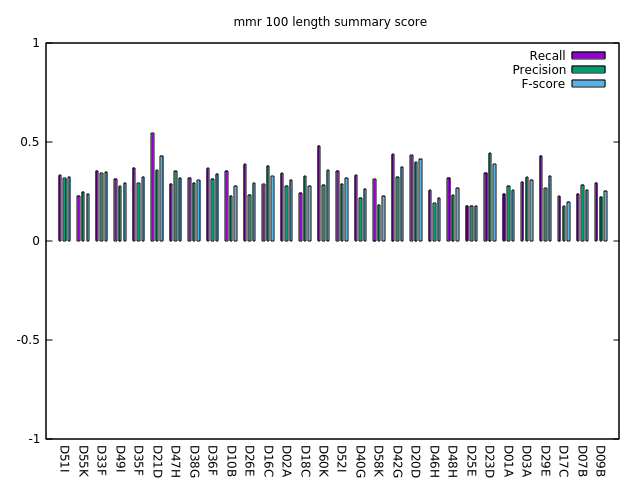
\includegraphics[scale=0.5]{IRReport/figure1.png}
\caption{Rouge score of MMR summary of length 100 words}
\label{fig:Result1}
\end{figure}

\begin{figure}[h!]
\centering
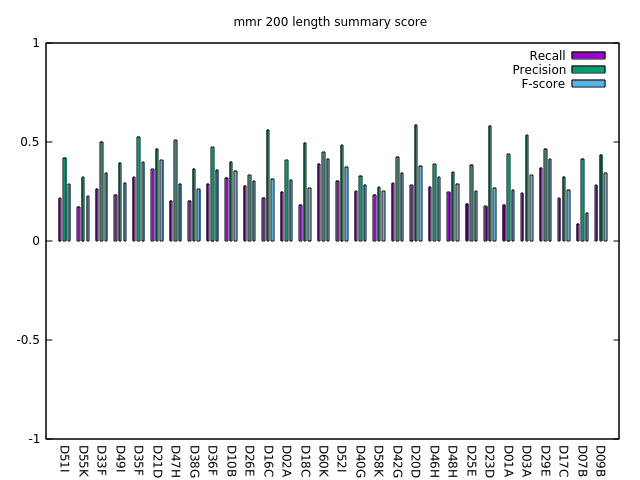
\includegraphics[scale=0.5]{IRReport/figure2.png}
\caption{Rouge score of MMR summary of length 200 words}
\label{fig:Result2}
\end{figure}


\begin{figure}[h!]
\centering
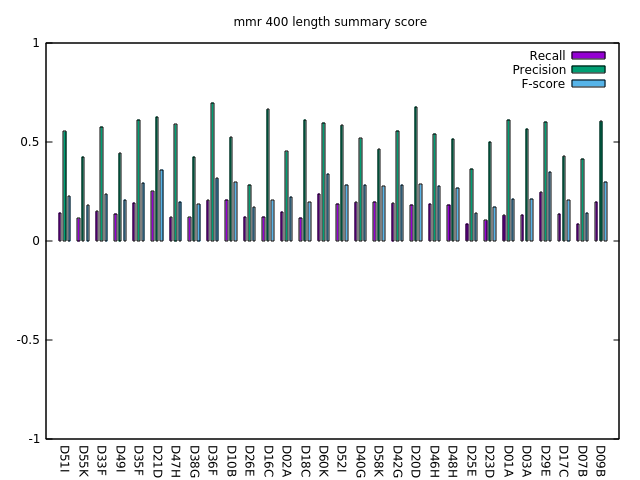
\includegraphics[scale=0.5]{IRReport/figure3.png}
\caption{Rouge score of MMR summary of length 400 words}
\label{fig:Result3}
\end{figure}
From figures [1][2][3] plot the rouge scores for document cluster of 30 documents of DUC2001 dataset. We see that MMR multi document text summarization technique provides an average recall of 34.8\%, average precision of 45.2\% and average F-score of 41.9\%. Average rouge score for our implementation of MMR summarization would be {34.8, 45.2, 41.9}. This is lower when compared to the average rouge score of original paper which was {44.8, 45.9, 45.83}, this is as the original paper uses normalized recall and F-score to provide better accuracy and use TF-IDF-ID instead of TF-IDF for sentence ranking. In best case scenario our approach has the rogue score of {60.2, 71.9, 47.8} this is similar to the original paper’s rogue score.
\par
We also observe that as the length of summary increases from 100 words to 400 words the recall value and f-score decrease while precision increases. Recall value is the total number of correct words that are present in summary versus total correct words, as the length of summary increases we probability of fetching incorrect words increases and as the number of sentences we pick to calculate MMR remains same the recall value is impacted. The same goes for f-score. However, precision is the total number of correct words in the summary versus total words in the summary, this means that when summary length increases most correct words could be included in summary, this leads to increase in precision value.
\par
Figure [4] is the plot comparing the polarity of sentences in MMR with Naïve tone biasing approach indicated in blue color and human summary without any tone bias dataset denoted in red color. MMR was implemented using ��=0.7 and summary chosen for evaluation was 400-word length summary provided in DUC2001 dataset. We see that few documents have negative polarity in human summary and MMR with naïve tone biasing successfully changes the polarity of all documents to positive polarity. We can observe that few document clusters find have negative polarity higher than positive polarity, this indicates that the document has high negative polarity and converting such document to positive polarity meant dropping lot of negative sentiment sentences which results in loss of information. 
\begin{figure}[h!]
\centering
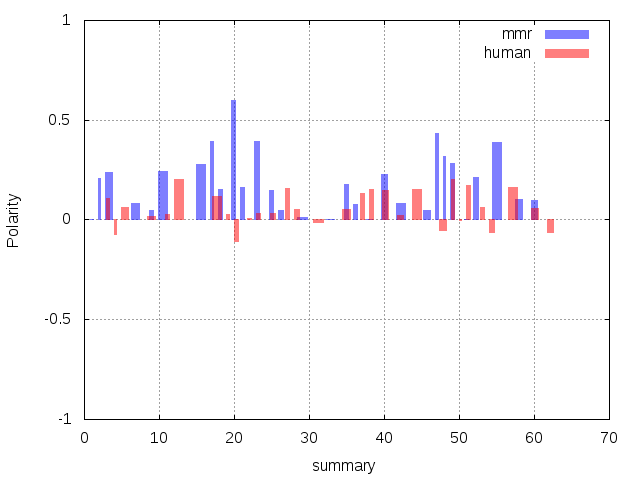
\includegraphics[scale=0.5]{IRReport/figure4.png}
\caption{Polarity of document clusters with and without tone biasing}
\label{fig:Result4}
\end{figure}


\section{Conclusion and Future Work}
We observed that MMR based multi-document text summarization provides good accuracy and is superior to other approaches removing redundant information in summary. Naïve tone biasing approach works well but might result in information loss when the tones we don’t need are too high in the document. Such loss of information can be mitigated by rephrasing sentences with required tone instead of discarding them this become a part of NLP problem and their future scope for us to work this area.

Naive tone biasing approach does binary biasing, i.e. either positive bias or negative bias and meaning of positive and negative might vary with the subject. As such instead of having a static lexicon of polarity scores of words we need develop a model to dynamically generate a lexicon with polarities according the subject. Such a model would give us better accuracy as the lexicon is customized to the subject/topic in point. Also, in some subjects/topics it might be better to have \textit{multiclass} biasing instead of having only two classes. We need to develop a model to identify different classes of information and construct a polarity lexicon.





\bibliographystyle{plain}
\bibliography{citation}
%\bibitem{IEEEhowto:kopka}
%H.~Kopka and P.~W. Daly, \emph{A Guide to \LaTeX}, 3rd~ed.\hskip 1em plus
%  0.5em minus 0.4em\relax Harlow, England: Addison-Wesley, 1999.






% that's all folks
\end{document}


